\section{Verifikáció és Validáció}

\subsection{V Modell}

	\begin{center}
		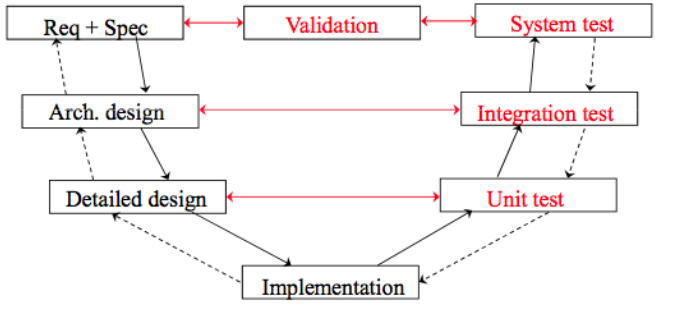
\includegraphics[scale=0.7]{img/vmodell}
	\end{center}

	\begin{enumerate}
		\item Unit test ( egységes teszt)
			\begin{itemize}
				\item Olyan elem, amit a programozó készít el.
				\item Alacsony szintű, de részletes teszt
				\item Elemekről szól ( 1-2 osztály OO esetén)
			\end{itemize}

		\item Integration test ( Integrációs teszt )
			\begin{itemize}
				\item Független tesztelők végzik/készítik
				\item A fő cél annak vizsgálata, hogy az egyes egységek jól működnek e
				\item Az egységek együtt jól működnek e ( interakció, kommunikáció)
				\item \textbf{Erre 2 stratégia van: }
					\begin{itemize}
						\item \textbf{top-down:} Föntről rakunk össze egy programot, pl grafikusan menű, majd utána a funkciók. - Teszt betétet használunk ( \textbf{test stub} )	\footnote{A még hiányzó alárendelt szoftver komponenst helyettesíti (pl: under construction weblap)}
						\item \textbf{bottom-up:} Alulról készülünk el elemekkel, alacsony szintű funkciókat/ metódusokat rakunk össze, majd építkezünk fel. Az a problémája az, hogy hiányzik a keret amiből az egészet tudjuk használni, ezért kénytelenek vagyunk egy teszt keretet ( \textbf{test bed } készíteni, amibe az eddigi elkészült elemeket tudjuk betenni
						%TODO Test bedről normális leírás
					\end{itemize}
			\end{itemize}

		\item System test ( rendszer teszt)
			\begin{itemize}
				\item Fókuszban a rendzer, hogy helyesen működik-e
				\item Megvizsgáljuk, hogy a rendszer képességeit, jellemzőit tudjuk-e mutatni
			\end{itemize}

		\item Elfogadási teszt (Acceptance test):
			\begin{itemize}
				\item Kész a program, mielőtt átadjuk a felhasználóknak azelőtt tesztelünk.
				\item Teljesen formálisan le van írva, hogy milyen teszteket kell végrehajtani - informális tesztek
				\begin{itemize}
					\item Alfa teszt
					Házon belüli ad-hoc vizsgálat, nincs előírás

					\item Béta teszt
						A fejlesztők kiadják valamilyen körben ( internetes béta változat), automatikus vagy manuális visszajelzés alapján keresi ahibákat, felelőssék nélkül adják ki
				\end{itemize}
			\end{itemize}
	\end{enumerate}
